\documentclass[aspectratio=169,t,11pt]{beamer}
\usepackage{slides,math}
\addbibresource{references.bib}

\title{Dynamic Treatment Effect Estimation with Interactive Fixed Effects and Short Panels}
\author{\texorpdfstring{Kyle Butts$^*$ and Nicholas Brown$\dagger$}{Kyle Butts and Nicholas Brown}}
\begin{document}

\begin{frame}[plain]
  \maketitle

  {\footnotesize\color{zinc600}
    $^*$University of Colorado Boulder\hspace{2mm}
    $\dagger$Queen's University
  } 

  \vspace{20mm}
  {\footnotesize
    \url{https://kylebutts.com/files/JMP.pdf}\\[-2mm]
    \url{https://kylebutts.com/files/JMP_slides.pdf}
  }
\end{frame}

\section{Motivation}

\begin{frame}{Motivation}
  Treatment is often targeted to places/units based on their economic trends:

  \begin{itemize}    
    \only<1->{
      \item New apartment construction \smcitep{asquith2021local,pennington2021does}
      \begin{itemize}
        \item Built in appreciating neighborhoods
      \end{itemize} 
    }

    \pause
    \item Walmart entry \smcitep{basker2005job,neumark2008effects}
    \begin{itemize}
      \item Open stores in areas with growing retail spending
    \end{itemize}

    \pause
    \item Place-based policies \smcitep{neumark2015place}
    \begin{itemize}
      \item Target places with declining labor markets 
    \end{itemize}
  \end{itemize}

  \bigskip\pause
  Standard difference-in-differences assumption of parallel trends is \emph{implausible}
\end{frame}

\begin{frame}{Motivation}
  In some settings, the causes of these trends are due to larger economic forces and not location-specific shocks:
  
  \begin{itemize}
    \item New apartment construction
    \begin{itemize}
      \item Changing preferences for walkable neighborhoods
    \end{itemize} 

    \pause
    \item Walmart entry
    \begin{itemize}
      \item Growing employment increases disposable income
    \end{itemize}

    \pause
    \item Place-based policies
    \begin{itemize}
      \item Decline of manufacturing hurting manufacturing hubs
    \end{itemize}
  \end{itemize}
\end{frame}

\begin{frame}{Modeling differential trends}
  This paper models differential trends using a \textbf{factor model} that is popular in the finance/macroeconomics literature:

  \begin{itemize}
    \item Each time period there is a set of \emph{unobservable} macroeconomic shocks that are common across units
    \item Units vary based on their \emph{unobservable} baseline characteristics in how impacted they are by the shocks
  \end{itemize} 
\end{frame}

% \begin{frame}{Modelling differential trends}
%   For example, think about estimating impact of new housing construction on neighborhood home prices:
%   \begin{itemize}
%     \item Shocks to demand occur every year
%     \item Neighborhoods have different characteristics and therefore vary in impact
%   \end{itemize}
% 
%   \bigskip
%   Since new apartments are created in neighborhoods that are appreciating, violate standard parallel trends
% \end{frame}

\begin{frame}{This paper}
  We propose a \textbf{class of imputation-style treatment effect estimators} under a \textbf{factor model}.

  \begin{itemize}
    \item Our `imputation' style estimator explicitly estimates the untreated potential outcome, $\zinc{y_{it}(0)}$, in the post-treatment periods 
    \begin{itemize}
      \item Same strategy as synthetic control and imputation estimator in difference-in-differences context \smcitep{Borusyak_Jaravel_Spiess_2021}
    \end{itemize}
    
    \pause
    \item A factor model allows treatment can be targeted based on a unit/location's exposure to common shocks 
    \begin{itemize}
      \item Violates standard parallel trends
    \end{itemize}
    
    \pause
    \item Our estimator is valid in small-$T$ settings and under treatment effect heterogeneity
  \end{itemize}
\end{frame}

\begin{frame}{Current approaches}{Standard factor model estimators}
  There are many factor model estimators that jointly estimate coefficients on treatment dummies and the factor model

  \pause\medskip
  \emph{Issues:} 
  \begin{itemize}
    \item Similar to the modern difference-in-differences literature \smcitep{Goodman-Bacon_2021,Borusyak_Jaravel_Spiess_2021,Callaway_Santanna_2021}, standard estimators would face problems with negative weighting under treatment effect heterogeneity
  \end{itemize}
\end{frame}

\begin{frame}{This paper}{}
  Our treatment effect estimators allows any $\sqrt{N}$-consistent estimate of the macroeconomic shocks to be used to generate consistent treatment effect estimates 
  
  \bigskip
  \begin{itemize}
    \item Unlocks a large econometric literature on factor model estimation and incorporates it into causal inference methods
    \begin{itemize}
      \item e.g. principal components, quasi-long differencing, common-correlated effects, etc.
    \end{itemize}
  \end{itemize}
\end{frame}

\begin{frame}{Current approaches}{Two-way Fixed Effect Imputation Estimator}
  \smcitet{Borusyak_Jaravel_Spiess_2021} and \smcitet{Gardner_2021} propose an `imputation' estimator for two-way fixed effects model:
  $$
    \zinc{y_{it}(0)} = \mu_i + \lambda_t + u_{it}
  $$
  \vspace{-\bigskipamount}
  \begin{enumerate}
    \item Estimate fixed effects using untreated/not-yet-treated observations ($d_{it} = 0$). Predict $y_{it}(0)$ out-of-sample for treated observations
    \item Average $y_{it} - \hat{y}_{it}(0)$ for treated observations
  \end{enumerate}

  \medskip\pause
  \emph{This paper extends this approach for factor models}
\end{frame}

\begin{frame}{Current approaches}{Covariates in two-way fixed effect model}\label{slide:current_approaches_cov}
  Extend model with a set of \emph{observable} characteristics to allow for $X_i$-specific trends
  \begin{equation*}
    \zinc{y_{it}(0)} = \mu_i + \lambda_t + X_i \beta_t + u_{it}
  \end{equation*}% 
  \begin{itemize}
    \item E.g. Demand shocks estimated by $\beta_t$ for neighborhood characteristics $X_i$
  \end{itemize}
  
  \pause\medskip
  \emph{Issues:}
  \begin{itemize}
    \item The researcher might not be able to \emph{observe} the underlying `exposure' variables
    
    \item Noisy measures of true `exposure' only partially control for the problem \smcitep{kejriwal2021efficacy}
  \end{itemize}

  \bottomleft{\hyperlink{slide:noisy_xi_simulations}{\beamergotobutton{Simulation Evidence}}}
\end{frame}

\begin{frame}{Current approaches}{Synthetic Control} 
  The synthetic control estimator constructs a `control unit' that has the same exposure to the macroeconomic trends (a form of imputation)
  
  \begin{itemize}
    \item Synthetic control is consistent when $\zinc{y_{it}(0)}$ has a factor model structure if you have a sufficiently large number of pre-periods 
  \end{itemize}

  \pause\medskip
  \emph{Issues:}
  \begin{itemize}
    \item In short-panels, you \emph{over-fit} on noise and get bad estimates \smcitep{abadie2010synthetic,ferman2021synthetic}
    
    \item Even if you have a large number of pre-periods, structural changes to the economy can make far-away pre-periods uninformative (e.g. the 2008 recession) \smcitep{abadie2021using}
  \end{itemize}
\end{frame}



\begin{frame}{Current approaches}{New synthetic-control style estimators}
  There are many estimators for treatment effects under factor models:
  \begin{enumerate}
    \item Synthetic control \smcitep{abadie2021using}
    \item Matrix Completion \smcitep{Athey_et_al_2021,bai2021matrix}
    \item Imputation Estimators \smcitep{Gobillon_Magnac_2016, Xu_2017}
  \end{enumerate}

  \bigskip
  \emph{None of these are valid in short-T settings.} Our paper introduces a general method that is valid in short-T settings.
\end{frame}

\begin{frame}{Current approaches}{Alternative short-$T$ factor model estimators}
  \smcitet{freyaldenhoven2019pre} propose a method that uses some variable $x_{it}$ that is affected by the same confounder that affects $y_{it}$ but not affected by treatment.
  \begin{itemize}
    \item This intuition is similar to a version of our estimator based on common-correlated effects \smcitep{Brown_Butts_Westerlund_2023}
    \item The estimator is not heterogeneity-robust
  \end{itemize}

  \bigskip
  \smcitet{Callaway_Karami_2020} propose a method for treatment effect estimation with a factor model
  \begin{itemize}
    \item The instrument they use would be valid for our quasi-long differencing estimator.
  \end{itemize}
\end{frame}

\begin{frame}{Preview of Application}{Impact of new Walmart entry on $\log$ retail employment. TWFE estimates}
  \vspace{-5mm}
  \begin{figure}
    \begin{adjustbox}{width=0.9\textwidth}
      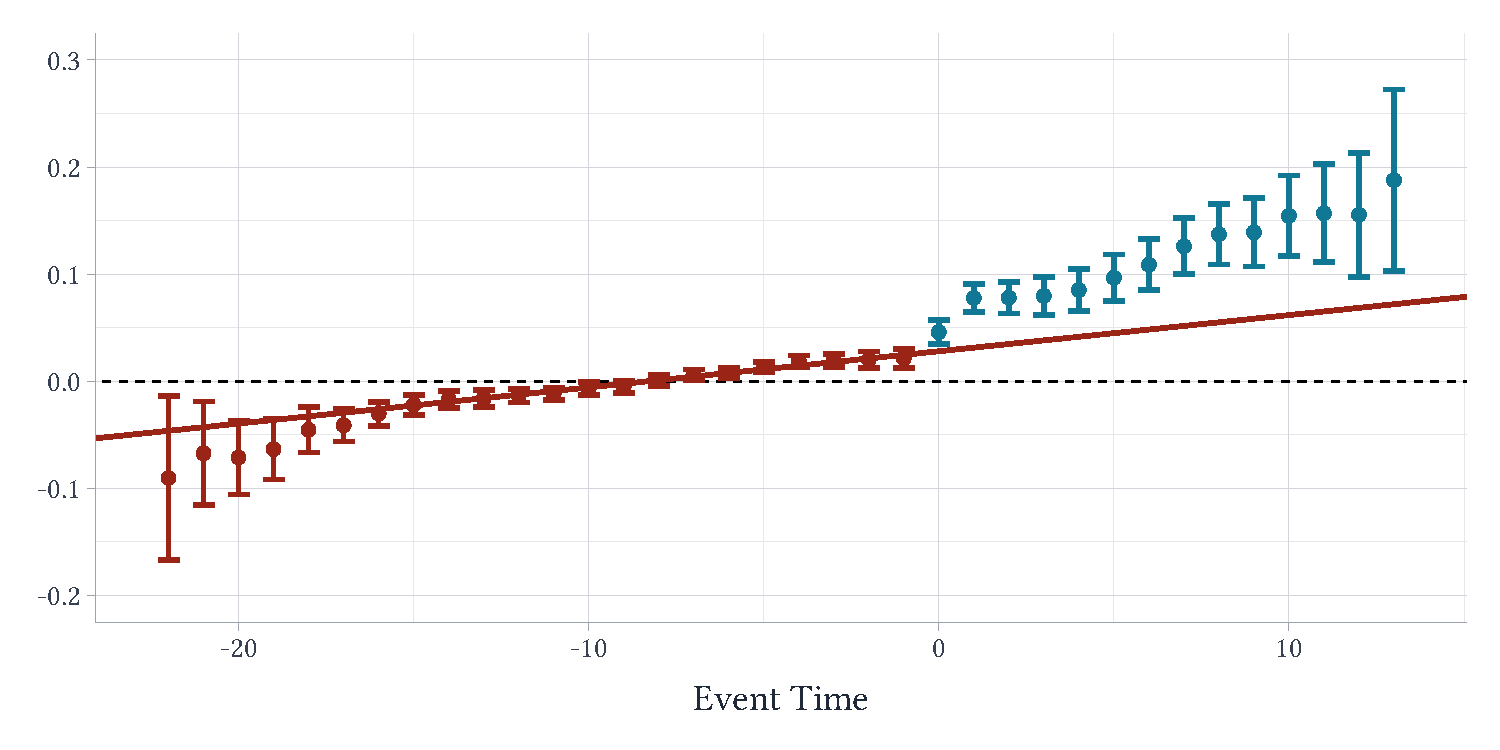
\includegraphics{../figures/did2s_retail.pdf}
    \end{adjustbox}
  \end{figure}
\end{frame}

\begin{frame}{Preview of Application}{Impact of new Walmart entry on $\log$ retail employment. Factor model estimates}
  \vspace{-5mm}
  \begin{figure}
    \begin{adjustbox}{width=0.9\textwidth}
      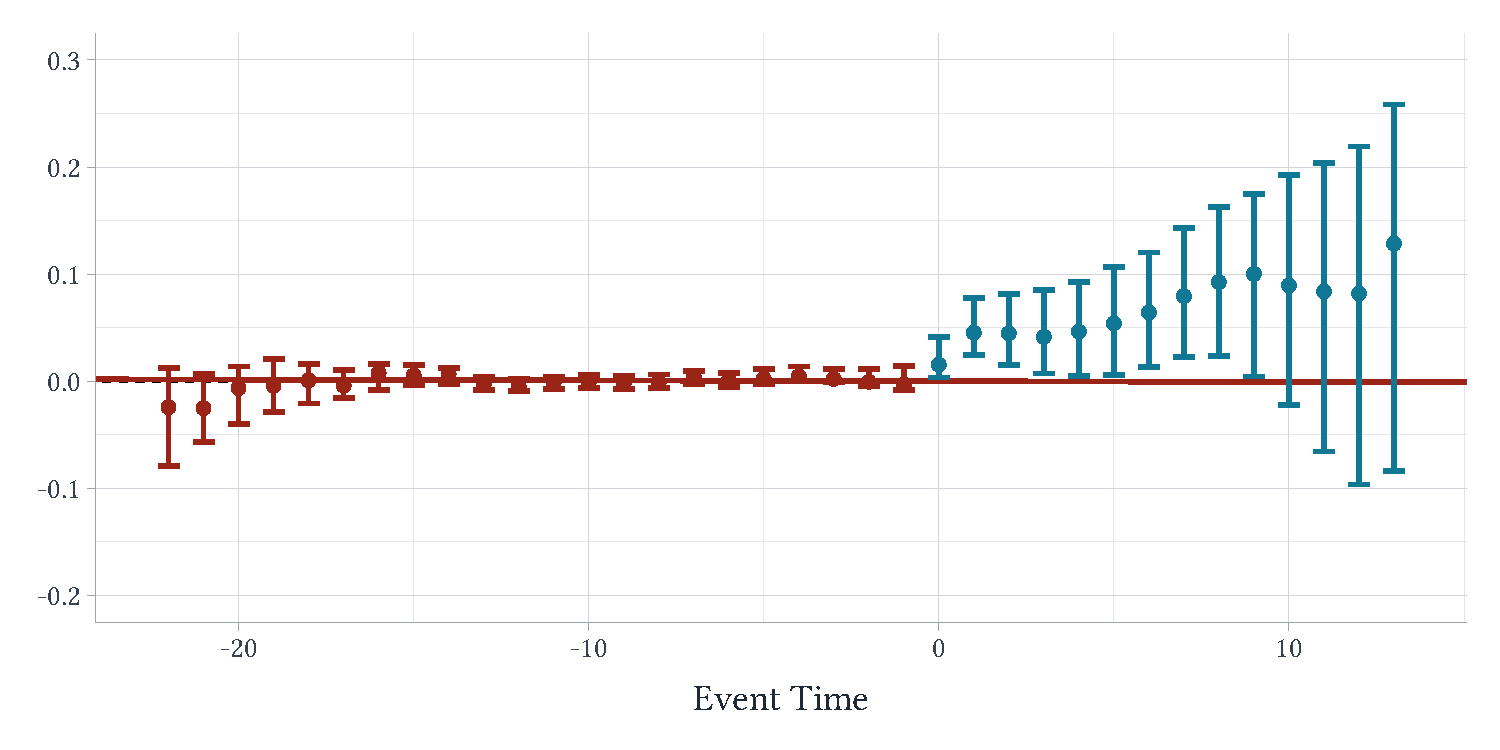
\includegraphics{../figures/qld_retail.pdf}
    \end{adjustbox}
  \end{figure}
\end{frame}

% \begin{frame}{Preview of Application}{Generalized method}
%   \vspace{-7.5mm}
%   \begin{figure}
%     \begin{adjustbox}{width=0.7\textwidth}
%       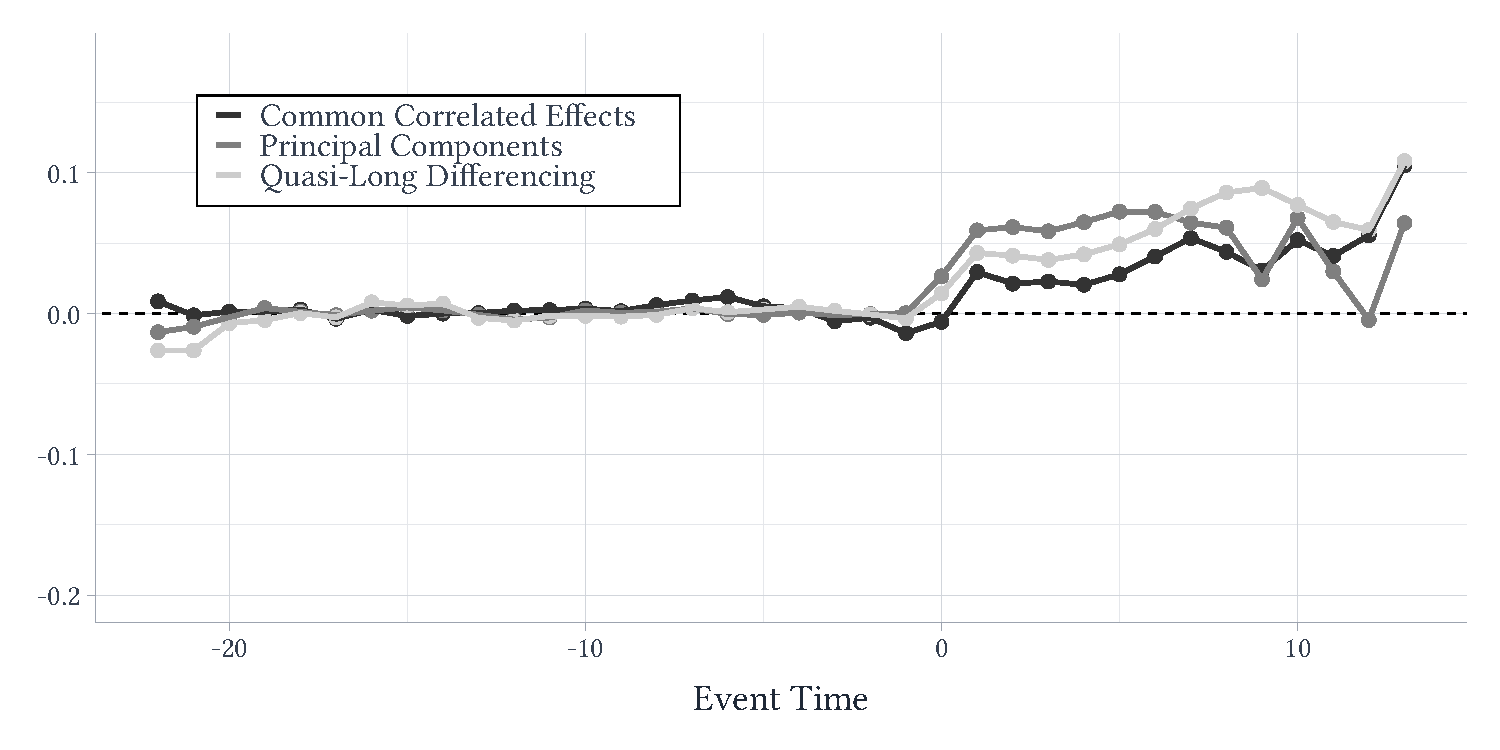
\includegraphics{../figures/retail_many_estimators.pdf}
%     \end{adjustbox}
%   \end{figure}
% 
%   Our method allows many estimators for the factor shocks
% \end{frame}

% \begin{frame}{Preview of Application}{Imputation estimator}
%   \vspace{-7.5mm}
%   \begin{figure}
%     \begin{adjustbox}{width=0.7\textwidth}
%       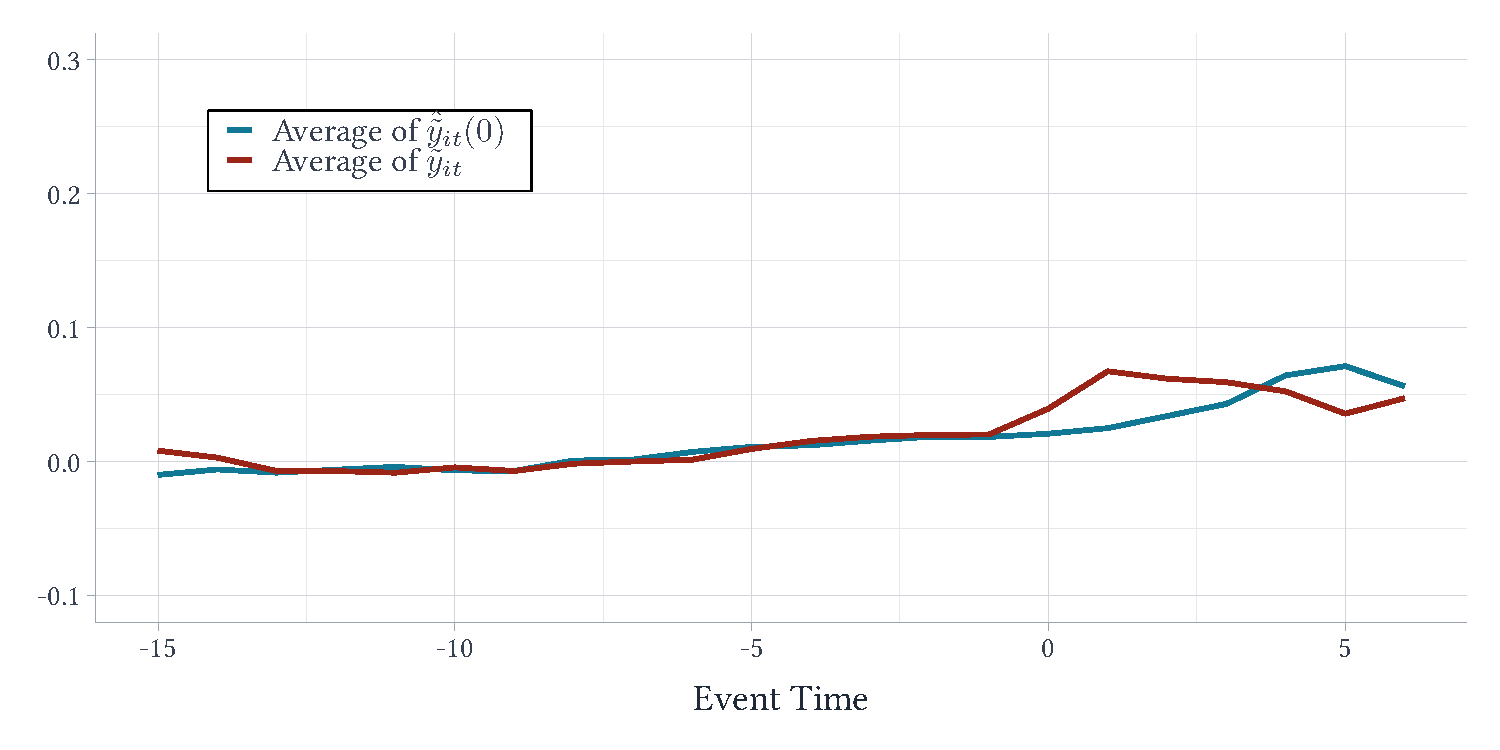
\includegraphics{../figures/synth_retail.pdf}
%     \end{adjustbox}
%   \end{figure}
% 
%   Our method "imputes" $y_{it}(0)$
% \end{frame}

\section{General Identification Result}

% \begin{frame}{Model}
%   \begin{block}{Assumption}
%     For $t = 1, \dots, T$: 
%     \begin{equation}
%       \expec{y_{it}(0)}{\gamma_i, D_i} = 
%     \end{equation}
% 
%   \end{block}
% 
% \end{frame}

\begin{frame}{Model}\label{slide:factor_model}
  We observe a panel of observations denoted by unit $i \in \{1, \dots, N\}$ and by time period $t \in \{1, \dots, T\}$. 
  
  \bigskip
  Untreated potential outcomes are given by a factor model:
  \begin{equation}\label{eq:untreated_po}
    y_{it}(0) = \sum_{r = 1}^{p} \purple{f_{t,r}} * \orange{\gamma_{i,r}} + u_{it}
  \end{equation}

  \begin{itemize}
    \item $f_{t, r}$ is the $r$-th \textbf{\color{purple} factor} (macroeconomic shock) at time $t$.
    \item $\gamma_{i,r}$ is unit i's \textbf{\color{orange} factor loading} (exposure) to the $r$-th factor.
  \end{itemize}

  \bottomleft{%
    \hyperlink{slide:appendix-selecting_p}{\beamergotobutton{Selecting $p$}} \ 
    \hyperlink{slide:appendix-shift_share}{\beamergotobutton{Differences with Shift-Share IV}}
  }
\end{frame}

\begin{frame}{Two-way Fixed Effect vs. Factor Model}
  The factor model is a generalization of the TWFE model. If $\bm{f}_{t} = (\lambda_t, 1)'$ and $\bm{\gamma}_i = (1, \mu_i)'$, then (\ref{eq:untreated_po}) becomes the TWFE model:
  $$
    y_{it}(0) = \bm{f}_t' \bm{\gamma}_i + u_{it} = \lambda_t + \mu_i + u_{it}
  $$
  
  \medskip
  Since TWFE is the work-horse model used by applied researchers, later we will explicitly add unit and time fixed-effects back in.
\end{frame}

\begin{frame}{Treatment Effects}
  For now, assume there is a single treatment that turns on in some period $T_0 + 1$. Define $D_i$ to be a dummy to denote which units receive treatment and $d_{it}$ to equal 1 when treatment is active.
  \begin{itemize}
    \item We assume $N_1 = \sum_i D_i$ and $N_0 = \sum_i D_i$ are non-vanishing as $N$ grows.
    \item $T_0 \geq p$ for identification
  \end{itemize}

  \pause\bigskip
  We are interested in event-study style average treatment effects. For each $t$, we define
  $$
    \text{ATT}_t \equiv \expec{y_{it}(1) - \zinc{y_{it}(0)}}{D_i = 1},
  $$
  where $\zinc{y_{it}(0)}$ is the (unobserved) untreated potential outcome.
\end{frame}

\begin{frame}{Assumptions}{Factor model}
  \vspace{-\medskipamount}
  \begin{block}{}
    \zinc{\textbf{Assumption:} Selection into Treatment}

    Untreated potential outcomes are given by 
    $$
      \zinc{y_{it}(0)} = \bm f_t' \bm{\gamma}_i + u_{it}.
    $$
    where $\expec{u_{it}}{\bm{\gamma}_i, D_i} = \expec{u_{it}}{\bm{\gamma}_i} = 0$ for all $t$.
  \end{block}
  
  \begin{itemize}
    \item Treatment can \emph{not} be correlated with unit-time specific shocks $u_{it}$ 
    
    \item Relaxes parallel trends by allowing units to enter treatment based on exposure to macroeconomic shocks
  \end{itemize}
\end{frame}

\begin{frame}{Assumptions}{Additional assumptions}
  \vspace{-\medskipamount}
  \begin{block}{}
    \zinc{\textbf{Assumption:} Arbitrary Treatment Effects}
    
    Treatment effects are left unrestricted (besides having finite moments):
    $$    
      \tau_{it} = y_{it}(1) - \zinc{y_{it}(0)}
    $$
  \end{block}

  \begin{block}{}
    \zinc{\textbf{Assumption:} No Anticipation}

    Whenever $d_{it} = 0$, the observed $y_{it} = \zinc{y_{it}(0)}$.
  \end{block}
\end{frame}

\begin{frame}{$\text{ATT}_t$ Identification}
  For a given $t$, our selection into treatment assumption implies:
  \begin{align*}
    \text{ATT}_t &\equiv \expec{y_{it}(1)}{D_i = 1} - \expec{y_{it}(0)}{D_i = 1} \\
    &= \expec{y_{it}(1)}{D_i = 1} - \expec{\bm{f}_t' \bm{\gamma}_i + u_{it}}{D_i = 1} \\
    &= \expec{y_{it}(1)}{D_i = 1} - \bm{f}_t' \expec{\bm{\gamma}_i}{D_i = 1}
  \end{align*}  

  \bigskip
  \textbf{Insight:} Estimating each $\bm{\gamma}_i$ requires large-$T$
  \begin{itemize}
    \item We only need to estimate $\expec{\bm{\gamma}_i}{D_i = 1}$ which is possible in small-$T$ settings
  \end{itemize}
\end{frame}

\begin{frame}{$\text{ATT}_t$ Identification}
  Suppose we observed the $T \times p$ matrix of factors, $\bm{F}$. Let `$\text{pre}$' denote the rows corresponding to $t \leq T_0$. Then for $t > T_0$,
  \begin{align*}
    &\expec{
      y_{it} - \bm{f}_t' (\bm{F}_{\text{pre}}' \bm{F}_{\text{pre}})^{-1} \bm{F}_{\text{pre}}'
      \underbrace{\bm y_{i,\text{pre}} }_{\bm{F}_{\text{pre}} \bm{\gamma}_i + \bm{u}_{i,\text{pre}}} 
    }{D_i = 1} \\
    &\quad = \expec{y_{it} - \bm{f}_t' \bm{\gamma}_i}{D_i = 1} \\
    &\quad = \expec{y_{it} - \zinc{y_{it}(0)}}{D_i = 1} = ATT_t,
  \end{align*}
  where the first equality comes from $\expec{u_{it}}{D_i = 1} = 0$.
\end{frame}

\begin{frame}{$ATT_t$ Identification}\label{slide:general_imputation_procedure}
  \vspace{-7.5mm}
  $$
    ATT_t = \expec{%
      y_{it} - \bm{f}_t' (\bm{F}_{\text{pre}}' \bm{F}_{\text{pre}})^{-1} \bm{F}_{\text{pre}}' \bm y_{i, \text{pre} } 
    }{D_i = 1} 
  $$

  \bigskip
  \emph{Technical Detail:}
  There is a well-known identification issue that $\bm{f}_t$ and $\bm{\gamma}_i$ are only known up to rotation: 
  
  E.g. $\bm{f}_t' \bm{\gamma}_i$ is the same multiply $\bm{f}_t$ by two and divide $\bm{\gamma}_i$ by two

  \pause
  \begin{itemize}
    \item This is no problem since our procedure produces numerically identical results for any rotation of $\bm{F}$ (OLS intuition).
    \item Hence, we only care about the column span of $\bm{F}$. 
  \end{itemize}

  \bottomleft{\hyperlink{slide:appendix-column_span_condition}{\beamergotobutton{Requirements for factor estimates, $\hat{\bm{F}}$}}}
\end{frame}

\begin{frame}{Estimation of $\bm{F}$}
  \vspace{-7.5mm}
  $$
    ATT_t = \expec{%
      y_{it} - \bm{f}_t' (\bm{F}_{\text{pre}}' \bm{F}_{\text{pre}})^{-1} \bm{F}_{\text{pre}}' \bm y_{i, \text{pre} } 
    }{D_i = 1} 
  $$

  \bigskip
  Consistency possible with $\sqrt{n}$-consistent estimation of the column-span of the factors $\bm{F}$.

  \smallskip
  \begin{itemize}
    \item This brings in a large literature on factor model estimation to causal-inference methods
    \begin{itemize}
      \item Will illustrate multiple estimators of $\bm{F}$ in application. 
    \end{itemize}
    
    \pause 
    \item Use only untreated observations, $D_{i} = 0$, for estimation of $\bm{F}$ to avoid bias.
    \item Staggered treatment `imputes' $y_{it}(0)$ separately for each treatment-timing group (changing $\text{pre}$)
  \end{itemize}
\end{frame}

\begin{frame}{Removing additive effects}\label{slide:remove_additive_fe}
  Now, we extend our base model to include additive effects
  $$
    y_{it} = \mu_i + \lambda_t + \bm{f}_t' * \bm{\gamma}_{i} + u_{it}
  $$
  
  We within-transform the outcome to remove the fixed effects:
  $$
    \tilde{y}_{it} = y_{it} - \overline{y}_{0,t} - \overline{y}_{i,pre} + \overline{y}_{0,pre}
  $$

  \bottomleft{%
    \hyperlink{slide:appendix-remove_additive_fe}{\beamergotobutton{Within-transform details}}
    \hyperlink{slide:twfe_test}{\beamergotobutton{Test for TWFE Model Sufficiency}}
  }
\end{frame}

\begin{frame}{Removing additive effects}
  \vspace{-\bigskipamount}
  $$
    \tilde{y}_{it} = y_{it} - \overline{y}_{0,t} - \overline{y}_{i,pre} + \overline{y}_{0,pre}
  $$

  \bigskip
  After performing our transformation, we have:
  $$
    \expec{\tilde{y}_{it}}{D_i = 1} = \expec{d_{it} \tau_{it} + \tilde{\bm f}_t' \tilde{\bm{\gamma}}_i }{D_i = 1}
  $$
  where $\tilde{\bm f}_t$ are the pre-treatment demeaned factors and $\tilde{\bm{\gamma}}_i$ are the never-treated demeaned loadings.

  \begin{itemize}
    \item \textbf{Novel result:} Our transformation removes $(\mu_i, \lambda_t)$ but preserves a common factor structure $\implies$ our imputation argument holds on transformed outcomes.
  \end{itemize}
\end{frame}

\section{Empirical Application}

\begin{frame}{Empirical Setting}
  We reevaluate the affect of Walmart openings on local labor markets. Mixed results in empirical literature \smcitep{basker2005job,neumark2008effects,basker2007good}.

  \pause\bigskip
  Walmart opens stores based on local economic trajectories.
  \begin{itemize}
    \item Plausibly, Walmart is not targeting a specific location based on local shocks, i.e. based on $u_{it}$

    \item Identification is based on assumption that Walmart picks places with growing retail sector due to national economic conditions, i.e. based on $\bm{f}_t' \bm{\gamma}_i$.
    \begin{itemize}
      \item Intuitively this is reasonable given Walmart's keg and spoke approach
    \end{itemize}
  \end{itemize}
\end{frame}

\begin{frame}{Data}
  We construct a dataset following the description in \smcitet{basker2005job}.

  \begin{itemize}
    \item In particular, we use the County Business Patterns dataset from 1964 and 1977-1999
    \item Subset to counties that (i) had more than 1500 employees overall in 1964 and (ii) had non-negative aggregate employment growth between 1964 and 1977
  \end{itemize}

  \smallskip\pause
  We use a geocoded dataset of Walmart openings from \smcitet{arcidiacono2020competitive}

  \begin{itemize}
    \item Treatment dummy is equal to one if the county has any Walmart in that year and our group variable denotes the year of entrance for the \emph{first} Walmart in the county.
  \end{itemize}
\end{frame}

\begin{frame}{Initial Estimates}
  To show problems with selection, we estimate a TWFE imputation model \smcitep{Wooldridge_2021,Borusyak_Jaravel_Spiess_2021}:
  \begin{equation}
      \log(y_{it}) = \mu_i + \lambda_t + \sum_{\ell = -22}^{13} \tau^\ell d_{it}^\ell + e_{it},
  \end{equation}
  \begin{itemize}
    \item $y_{it}$ include county-level retail employment and wholesale employment.
    \item $d_{it}^\ell$ are event-time dummies for being $\ell$ years away from when the initial Walmart opens in a county.
  \end{itemize}
\end{frame}

\begin{frame}
  \begin{figure}
    \caption{Effect of Walmart on County $\log$ Retail Employment (TWFE Estimate)}
    \begin{adjustbox}{width=0.85\textwidth}
      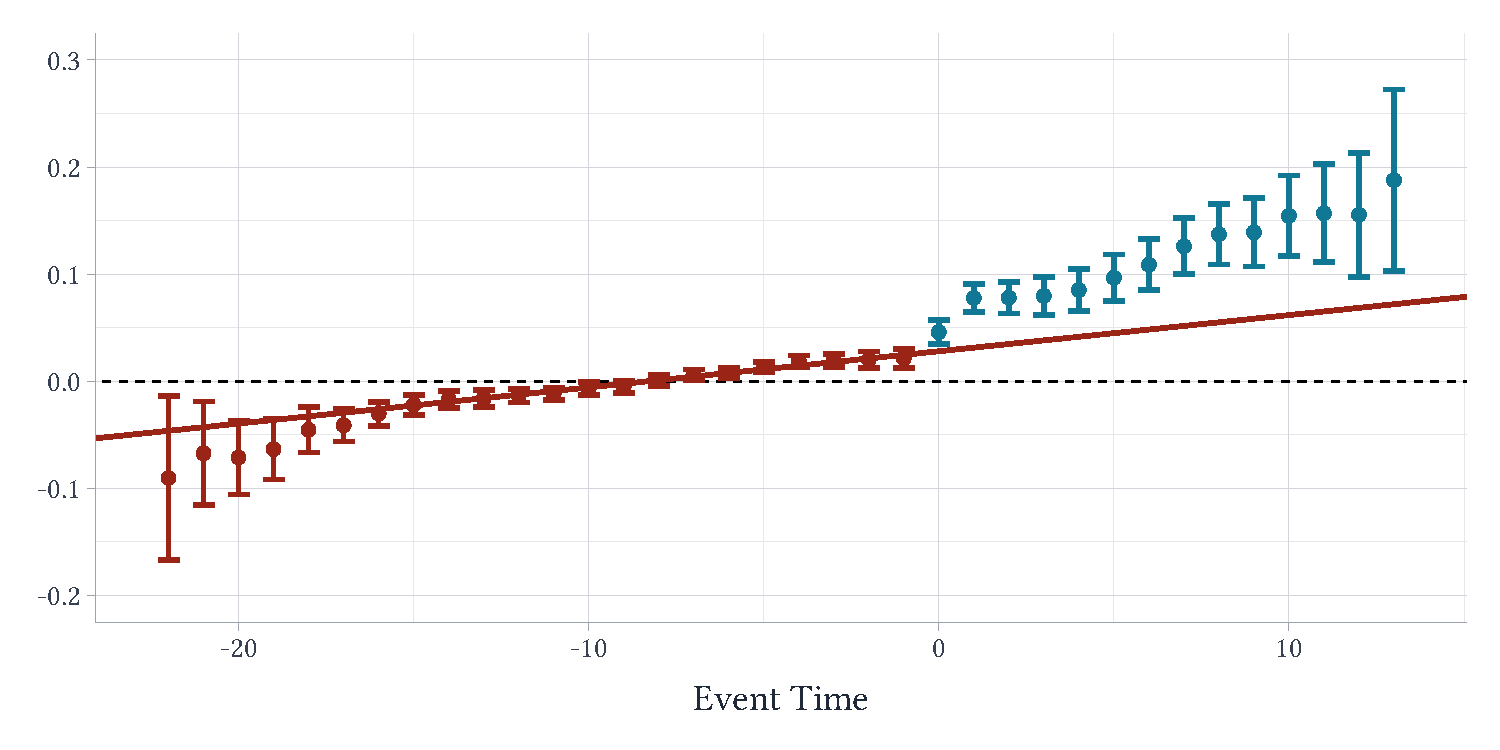
\includegraphics{../figures/did2s_retail.pdf}
    \end{adjustbox}
  \end{figure}
\end{frame}

\begin{frame}
  \begin{figure}
    \caption{Effect of Walmart on County $\log$ Wholesale Employment (TWFE Estimate)}
    \begin{adjustbox}{width=0.85\textwidth}
      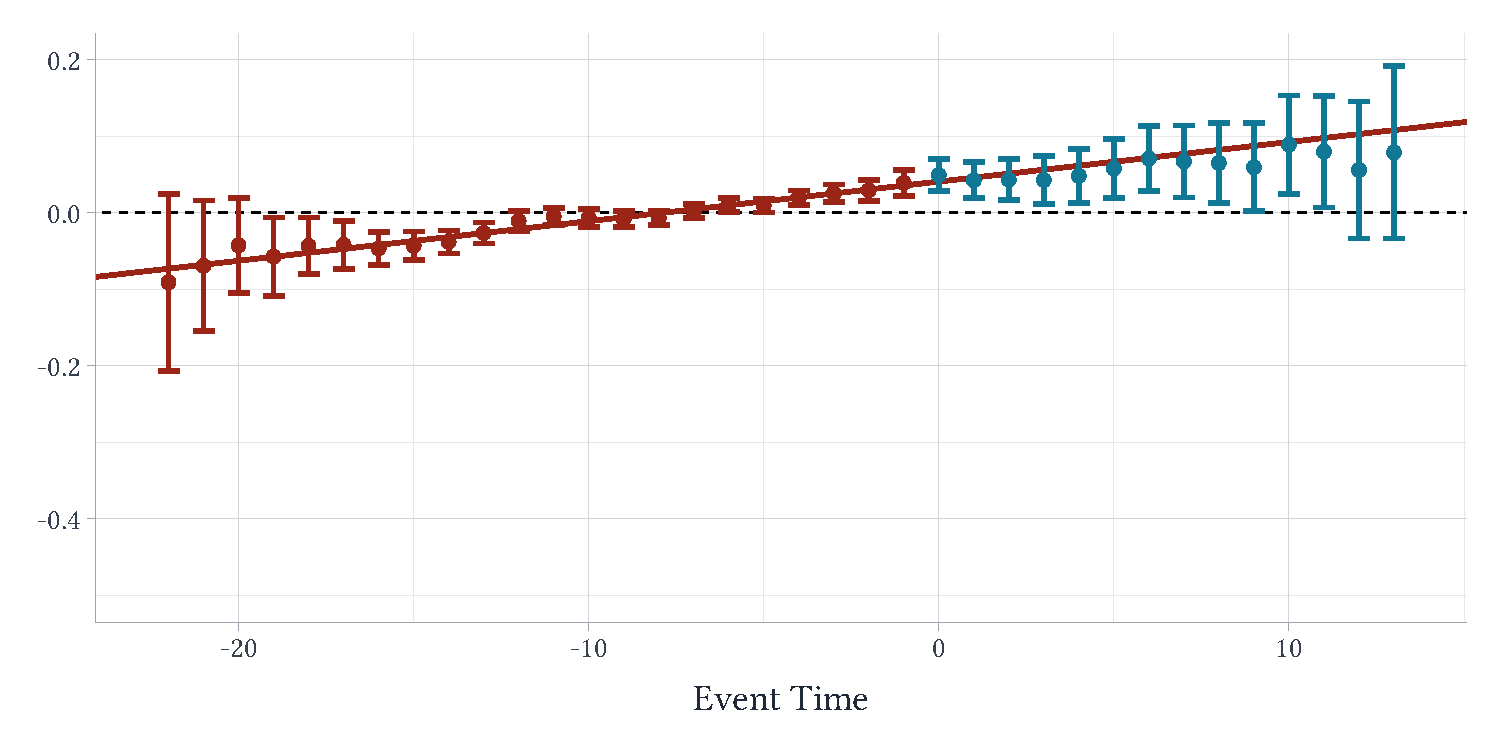
\includegraphics{../figures/did2s_wholesale.pdf}
    \end{adjustbox}
  \end{figure}
\end{frame}

\begin{frame}{Factor Identification}{Strategy 1: IV strategy}\label{slide:qld_strategy}
  We consider instrumental-variables based identification strategy as proposed in \smcitet{Ahn_Lee_Schmidt_2013}.
  \begin{itemize}
    \item Allows fixed-$T$ identification of $\bm{F}$.
    \item A GMM estimator $\implies$ inference is standard (derivation in paper)
  \end{itemize}

  \bottomleft{\hyperlink{slide:appendix-qld_details}{\beamergotobutton{Quasi-long Differencing Details}}}
\end{frame}

\begin{frame}{Factor Identification}{Strategy 1: IV strategy}
  Intuitively, we need a set of instruments that we think:

  \begin{itemize}
    \item {\color{zinc500} (Relevancy)} Are correlated with the factor-loadings $\gamma_i$.

    \item {\color{zinc500} (Exclusion)} Satisfy an exclusion restriction on $u_{it}$. We can't pick up on $(i,t)$ shocks that are correlated with treatment
  \end{itemize}

  \bigskip
  We think the best IV strategy entails using time-invariant characteristics $X_i$ that we think are correlated with $\gamma_i$

  \bottomleft{\hyperlink{slide:appendix-qld_details}{\beamergotobutton{Quasi-long Differencing Details}}}
\end{frame}

\begin{frame}{Factor Model}
  Turning to our factor model estimator, we use the following variables at their 1980 baseline values as instruments:
  \begin{itemize}
    \item share of population employed in manufacturing
    \item shares of population below and above the poverty line
    \item shares of population employed in the private-sector and by the government
    \item shares of population with high-school and college degrees
  \end{itemize}

  \smallskip\pause
  Think that these are predictive of the kinds of economic trends Walmart may be targeting
  \begin{itemize}
    \item Using baseline values helps us avoid picking up on concurrent shocks that are correlated with Walmart opening
  \end{itemize}
\end{frame}

\begin{frame}{}
  \vspace{-\bigskipamount}
  \begin{figure}
    \caption{Effect of Walmart on County $\log$ Retail Employment (Factor Model)}
    \begin{adjustbox}{width=0.85\textwidth}
      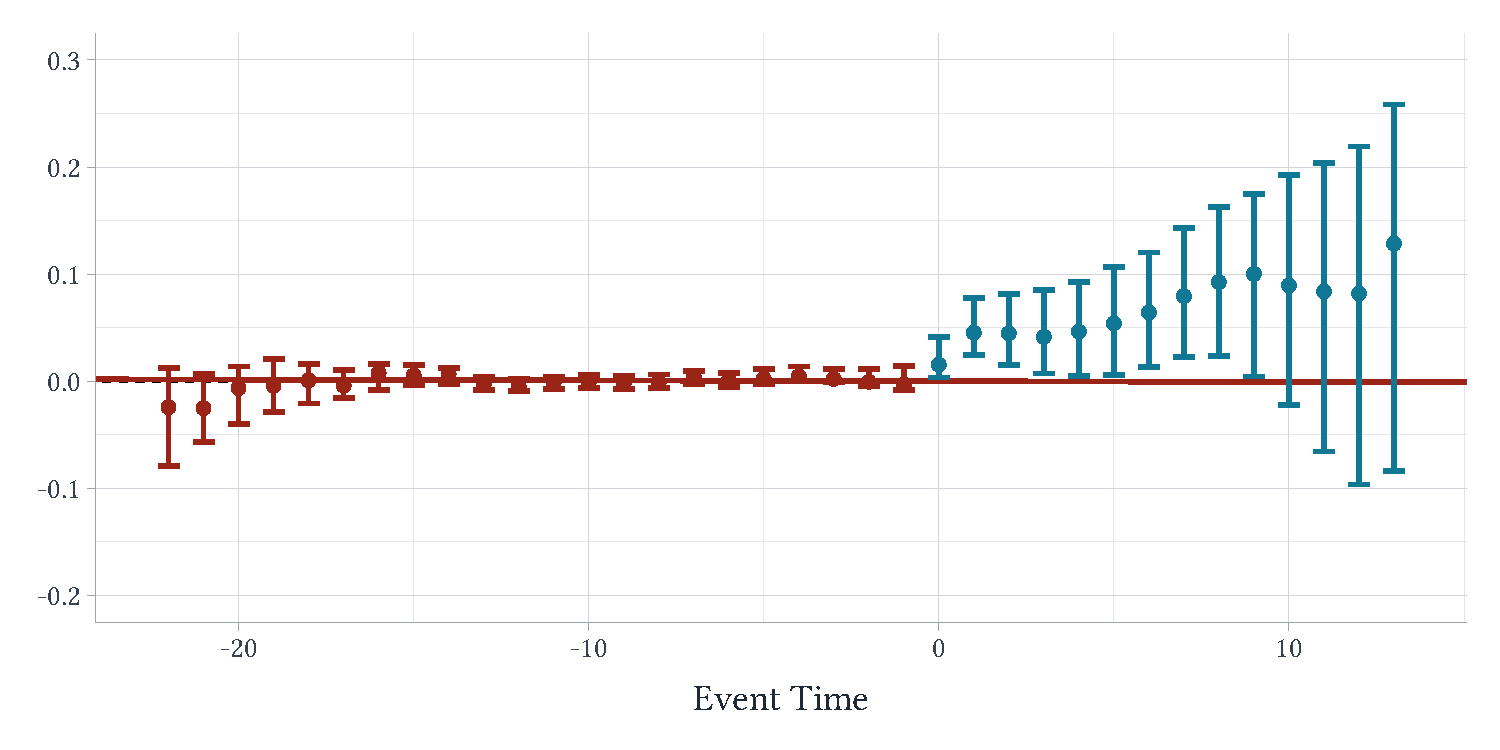
\includegraphics{../figures/qld_retail.pdf}
    \end{adjustbox}
  \end{figure}

  Increase of retail employment $\approx$ 5\%, consistent with \smcitet{basker2005job} and \smcitet{stapp2014walmart}
\end{frame}

\begin{frame}{}
  \vspace{-\bigskipamount}
  \begin{figure}
    \caption{Including instruments as $X_i \beta_t$ in TWFE Model}
    \begin{adjustbox}{width=0.9\textwidth}
      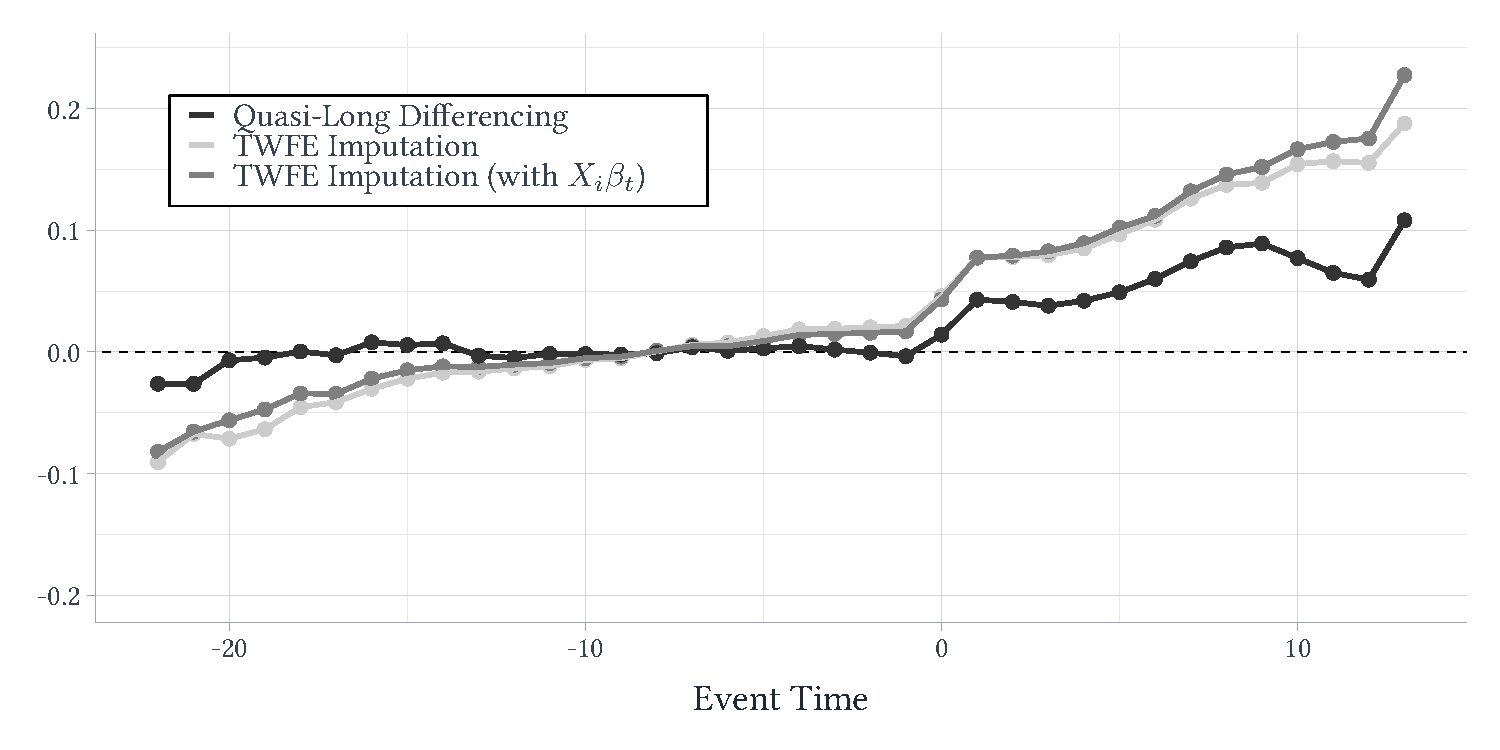
\includegraphics{../figures/retail_covs.pdf}
    \end{adjustbox}
  \end{figure}
\end{frame}

\begin{frame}{}
  \vspace{-\bigskipamount}
  \begin{figure}
    \caption{Effect of Walmart on County $\log$ Retail Employment (Factor Model)}
    \begin{adjustbox}{width=0.85\textwidth}
      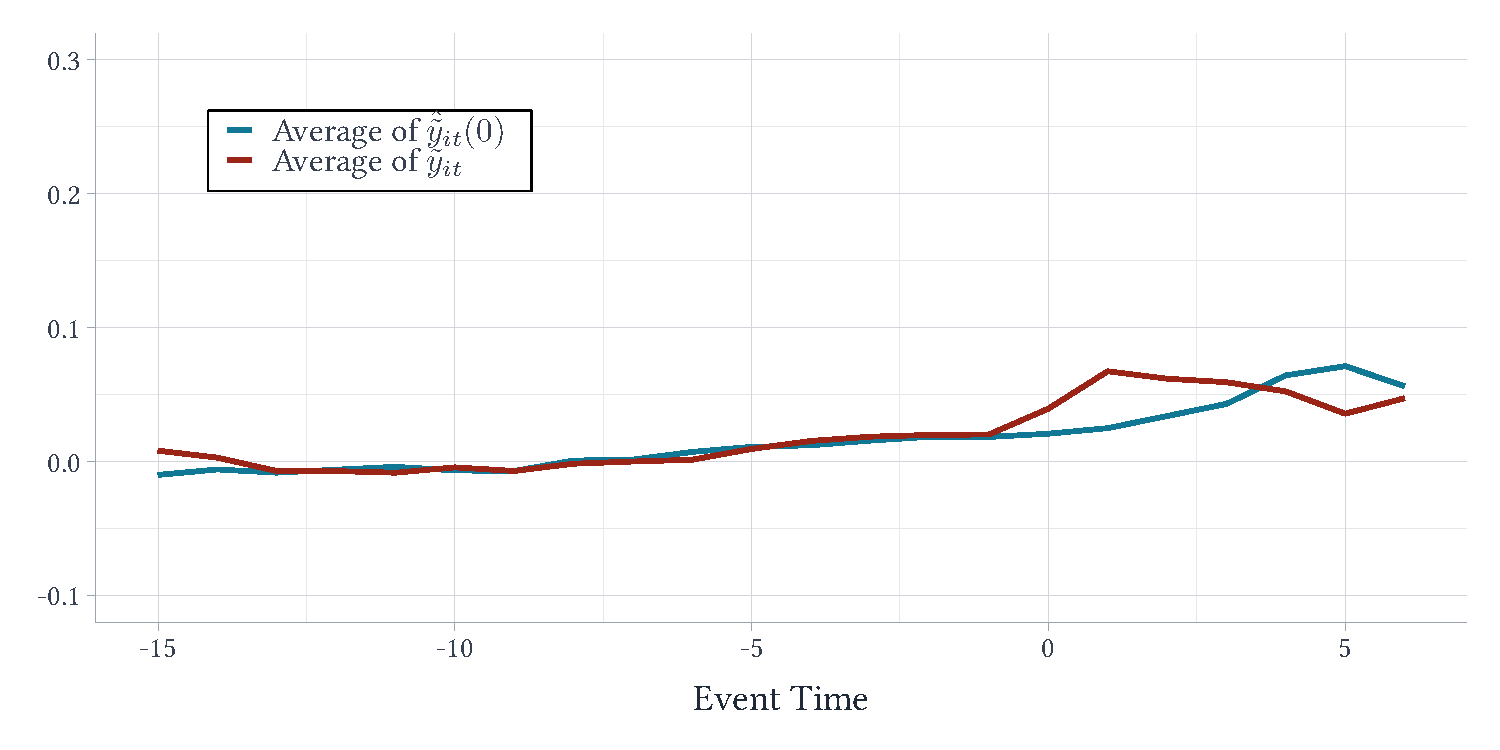
\includegraphics{../figures/synth_retail.pdf}
    \end{adjustbox}
  \end{figure}
\end{frame}


\begin{frame}{}
  \vspace{-\bigskipamount}
  \begin{figure}
    \caption{Effect of Walmart on County $\log$ Wholesale Employment (Factor Model)}
    \begin{adjustbox}{width=0.85\textwidth}
      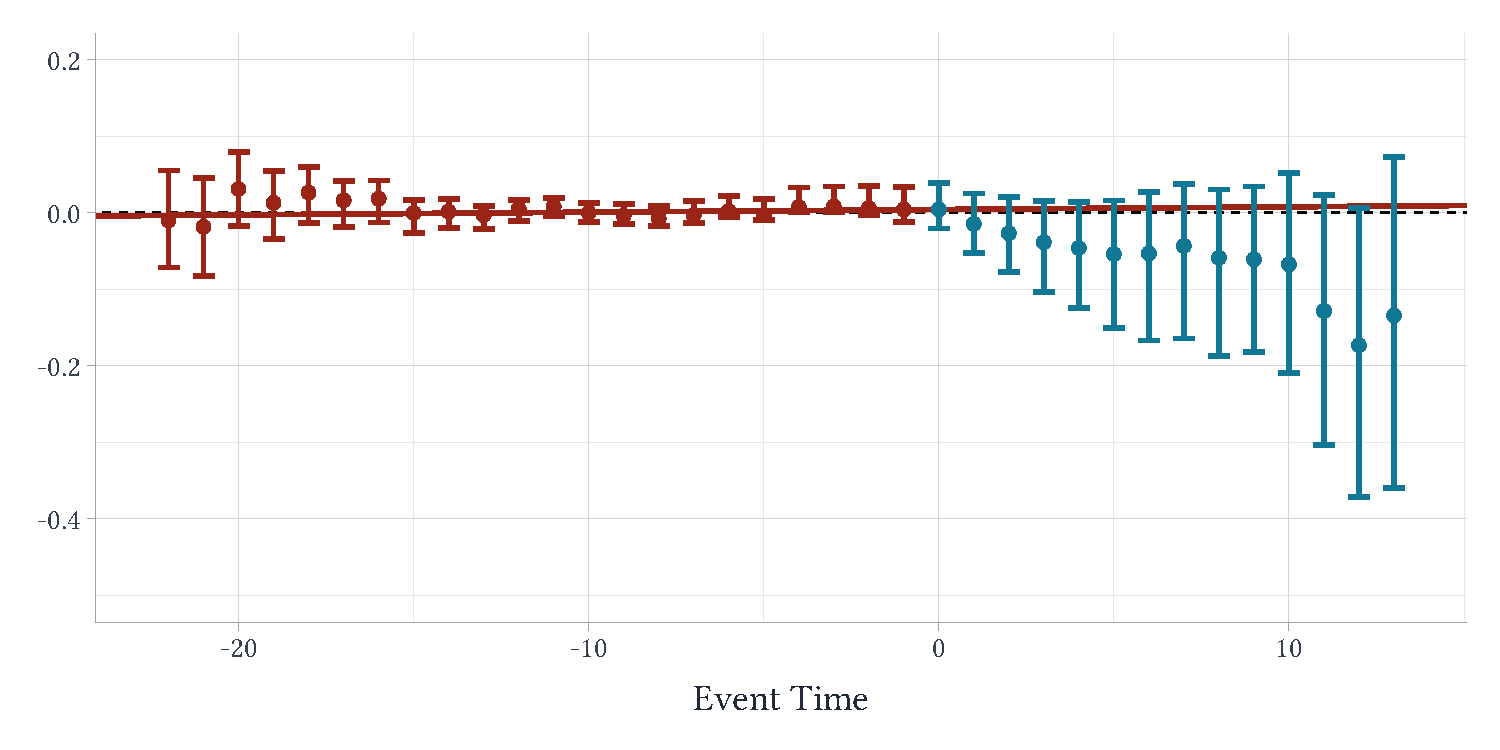
\includegraphics{../figures/qld_wholesale.pdf}
    \end{adjustbox}
  \end{figure}

  Very noisy, but consistent with estimates in \smcitet{basker2005job}.
\end{frame}

\begin{frame}{Alternative identification strategies}{Strategy 2: Principal Components}\label{slide:pc_strategy}
  An alternative identification strategy is a principal component decomposition of outcomes. 
  \begin{itemize}
    \item This method requires no additional variables
    \item Requires either a large number of pre-periods \smcitep{Xu_2017} or error term $u_{it}$ to not be autocorrelated \smcitep{Imbens_Kallus_Mao_2021}
  \end{itemize} 

  \bottomleft{
    \hyperlink{slide:appendix-pc_details}{\beamergotobutton{Principal Components Details}}
  }
\end{frame}

\begin{frame}{Alternative identification strategies}{Strategy 3: Common Correlated Effects}\label{slide:cce_strategy}
  The common correlated effects estimate is based on the availability of a set of additional covariates $\bm{x}_{it}$ that are affected by the same factors as $y_{it}$ \smcitep{pesaran2006estimation,freyaldenhoven2019pre}
  
  \begin{itemize}
    \item Cross-sectional averages of $\bm{x}_{it}$ across never-treated $i$ become proxies $\hat{\bm{F}}_t$. Need $\geq p$ covariates \smcitet{Brown_Butts_Westerlund_2023}.
  \end{itemize}

  \bigskip
  In our Walmart setting, we use the log employment for the manufacturing, construction, agriculture, and healthcare 2-digit NAICS codes for $\bm{x}_{it}$

  \bottomleft{
    \hyperlink{slide:appendix-cce_details}{\beamergotobutton{Common Correlated Effects Details}} \ 
    \hyperlink{slide:appendix-wto_application}{\beamergotobutton{CCE and Mediated Effects}}
  }
\end{frame}

\begin{frame}{}
  \vspace{-\bigskipamount}
  \begin{figure}
    \caption{Generalized Procedure allows many factor estimators}
    \begin{adjustbox}{width=0.9\textwidth}
      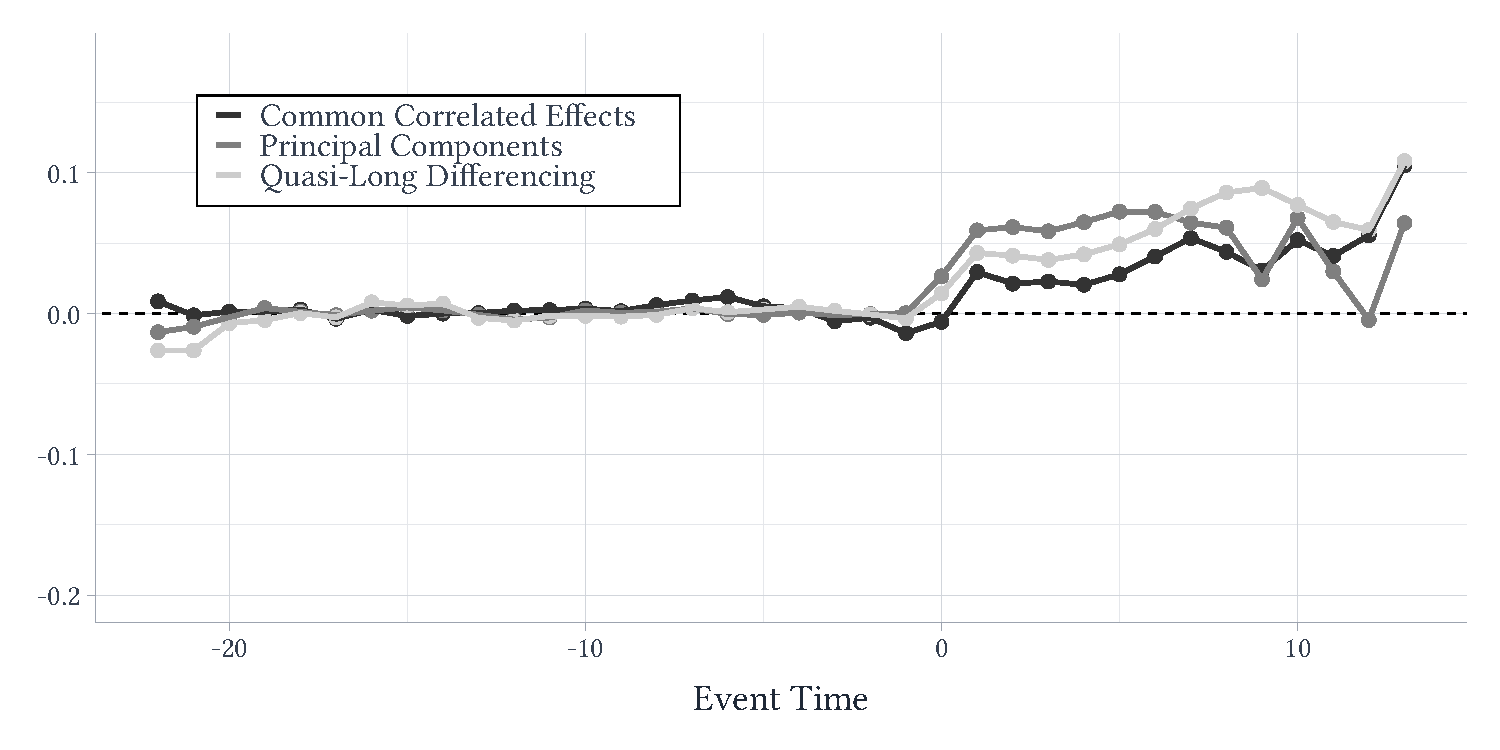
\includegraphics{../figures/retail_many_estimators.pdf}
    \end{adjustbox}
  \end{figure}
\end{frame}

\begin{frame}{Conclusion}
  Provide general identification results for ATTs under linear factor models. 
  \begin{itemize}
      \item Generalizes the two-way fixed effect model and is estimable in short-$T$ settings
      \item Can use multiple estimators for the factor space. 
      \begin{itemize}
          \item Brown et al. (2023) for CCE.
      \end{itemize}
  \end{itemize}

  \bigskip
  Implement quasi-long-differencing estimator
  \begin{itemize}
      \item Find results on Walmart's affect on local labor markets similar to Basker (2005). 
  \end{itemize}
\end{frame}

% ------------------------------------------------------------------------------
\begin{frame}[allowframebreaks]{References}
  \printbibliography
\end{frame}
\appendix
% ------------------------------------------------------------------------------



\begin{frame}{}\label{slide:noisy_xi_simulations}
  \begin{figure}
    \caption{TWFE model with noisy proxy variable $w_i = \gamma_i + v_i$}
    \begin{adjustbox}{width=0.9\textwidth}
      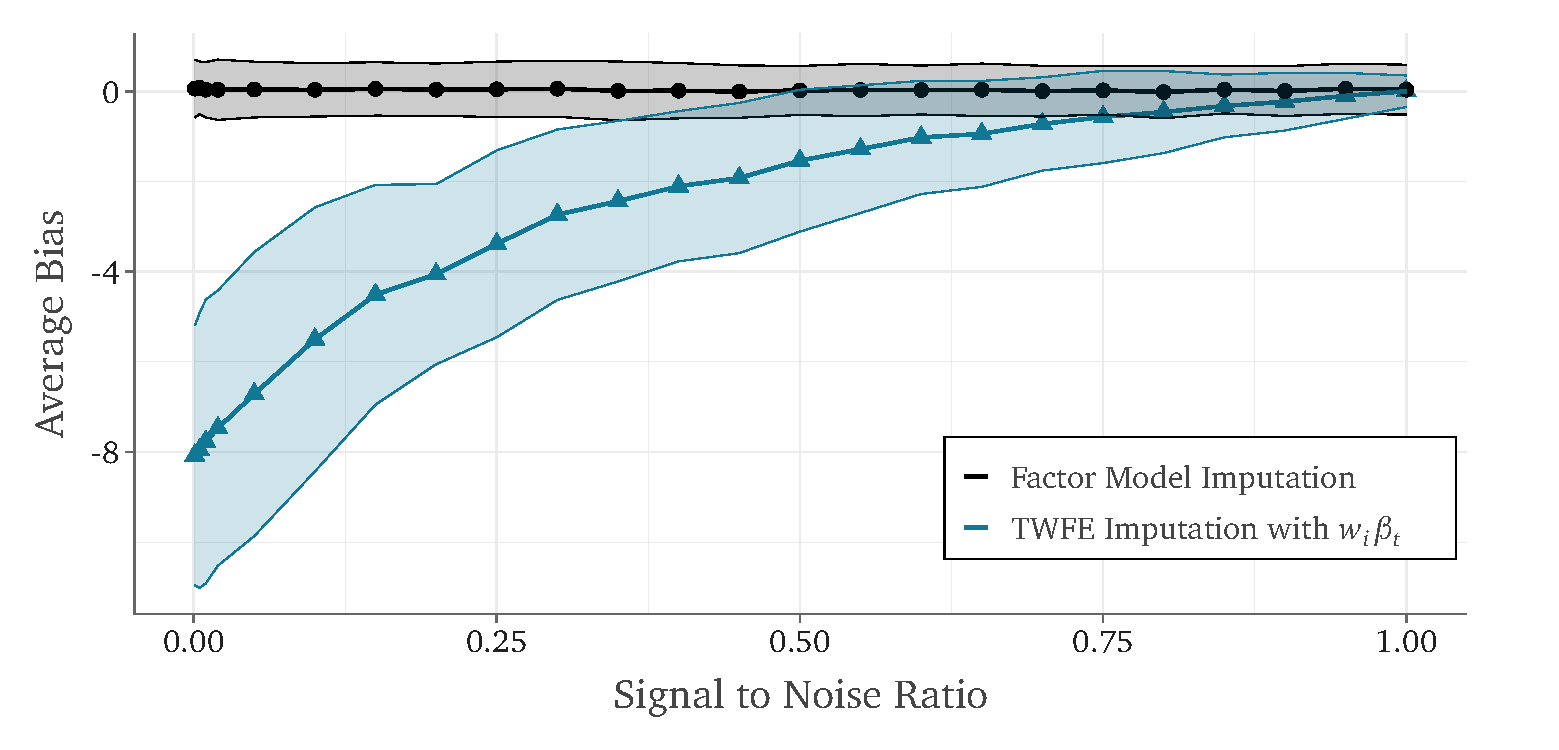
\includegraphics{../figures/simulation-bias_signal_to_noise.pdf}
    \end{adjustbox}
  \end{figure}
  
  \bottomleft{
    \hyperlink{slide:current_approaches_cov}{\beamergotobutton{Back}}
  }
\end{frame}

\begin{frame}{Intuition of Factor Model}\label{slide:appendix-shift_share}
  The intuition is very similar to that of the construction of a shift-share variable:
  $$
    z_{it} = \sum_{r = 1}^{p} f_{t,r} * \gamma_{i,r}
  $$
  \vspace{-5mm}
  \begin{itemize}
    \item The $p \times 1$ vector $\bm{f}_t$ is the set of \emph{`macroeconomic'} shocks (shifts) that all units experience
    \item $\bm{\gamma}_i$ is an individuals \emph{exposure} (shares) to the shocks 
  \end{itemize}

  \bigskip
  The difference being that \textbf{we do not observe} the variables $\bm{\gamma}_i$ and $\bm{f}_t$ (like we don't observe fixed effects)

  \bottomleft{\hyperlink{slide:factor_model}{\beamergotobutton{Model}}}
\end{frame}
  
\begin{frame}{Removing additive effects}\label{slide:appendix-remove_additive_fe}
  We consider the residuals after within-transforming
  $$
    \tilde{y}_{it} = y_{it} - \overline{y}_{0,t} - \overline{y}_{i,pre} + \overline{y}_{0,pre},
  $$
  where
  \begin{gather*}
    \overline{y}_{i, pre} = \frac{1}{T_0} \sum_{t = 1}^{T_0} y_{it}, \qquad
    \overline{y}_{0, t} = \frac{1}{N_{0}} \sum_{i = 1}^N (1 - D_i) y_{it}, \qquad
    \overline{y}_{0, pre} = \frac{1}{T_0} \sum_{t = 1}^{T_0} y_{0, t}
  \end{gather*}

  \bottomleft{ 
    \hyperlink{slide:remove_additive_fe}{\beamergotobutton{Back}}
  }
\end{frame}

\begin{frame}{Test for TWFE Model}\label{slide:twfe_test}
  The ATTs are identified by the modified TWFE transformation if
  \begin{equation}\label{eq:twfe_loading_equality}
    \expec{\bm{\gamma}_i}{D_i} = \expec{\bm{\gamma}_i}
  \end{equation}
  For $t > T_0$
  $$
    \expec{\tilde{y}_{it}}{D_i = 1} = \expec{\tau_{it}}{D_i = 1} = \tau_t
  $$
  
  \begin{itemize}
    \item Says TWFE is sufficient even if there are factors, so long as exposure to these factors are the same between treated and control group.
  \end{itemize}

  
  \medskip
  In the paper, we provide tests for (\ref{eq:twfe_loading_equality}) under the quasi-long differencing identification strategy

  \bottomleft{
    \hyperlink{slide:remove_additive_fe}{\beamergotobutton{Back}}  
  }
\end{frame}

\begin{frame}{Factor Identification}\label{slide:appendix-column_span_condition}
  We cannot identify $\bm F$ or $\bm{\gamma}_i$ separately from one another. 
  \begin{itemize}
    \item Rotation problem means we can only identify $A \bm F$ for some matrix $A$.
  \end{itemize}

  \medskip
  Consider some estimator $\bm{F}(\theta)$ such that the true factor matrix $\bm{F} \in \text{col}(\bm{F}(\theta))$
  \begin{itemize}
    \item \textbf{Examples:} common correlated effects, principal components, quasi-differencing.
  \end{itemize}

  \smallskip
  Then using $\bm{F}(\theta)$ in place of $\bm{F}$ still identifies $\text{ATT}_t$.
  \begin{itemize}
    \item $\bm{f}_t (\bm{F}_{\text{pre}}' \bm{F}_{\text{pre}})^{-1} \bm{F}_{\text{pre}}$ is invariant to rotating by any invertible matrix $A \bm{F}$.
  \end{itemize}

  \bottomleft{\hyperlink{slide:general_imputation_procedure}{\beamergotobutton{Back}}}
\end{frame}


\begin{frame}{Quasi-long Differencing Details}\label{slide:appendix-qld_details}
  The quasi-long differencing method \citet{Ahn_Lee_Schmidt_2013} normalize the factors:
  \begin{equation*}
    \bm{F}(\bm{\theta}) = 
    \begin{pmatrix}
        -\bm I_p \\
        \bm \Theta
    \end{pmatrix}
  \end{equation*}

  \begin{itemize}
    \item Recall, this normalization does not impact imputation.
  \end{itemize}

  Quasi-differencing transformation: $\bm H(\bm \theta) = [\bm \Theta, \bm I_{(T-p)}]$. For all $\theta$, we have
  $$
    \bm{H}(\bm{\theta}) \bm{F}(\bm{\theta}) = 0
  $$

  \bottomleft{\hyperlink{slide:qld_strategy}{\beamergotobutton{Back}}}
\end{frame}

\begin{frame}{Factor Identification}
  This transformation creates a set of moments:
  $$
    \expec{\bm{W}_i' \bm{H}(\bm{\theta}) \bm{y}_i}{D_i = 0}
  $$

  \begin{itemize}
    \item $W_i$ is a $(T - p) \times w$ matrix of instruments ($w \geq p$).
    \item $W_i$ must be exogenous after removing factors.
    \item $\hat{\bm{\theta}}$ is Fixed-$T$ consistent.
  \end{itemize}

  \bottomleft{\hyperlink{slide:qld_strategy}{\beamergotobutton{Back}}}
\end{frame}

\begin{frame}\label{slide:appendix-general_factor}
  \begin{block}{}
    \zinc{\textbf{Assumption:} General framework for factor estimators}

    There exists a $q \times 1$ vector of paramters $\bm{\theta}$ and a $T \times m$ function $\bm{F}(\bm{\theta})$ such that the following conditions hold:
    \begin{enumerate}
      \item[(i)] For some full-rank matrix $\bm{A}$, $\bm{F}(\bm{\theta}) \bm{A} = \bm{F}$ where $\text{Rank}(\bm{F}(\bm{\theta})) = m < T_0$ 
      \item[(ii)] There is a $s \times 1$ vector of moment functions $\bm g_{i\infty}(\bm{\theta})$ such that 
      \begin{equation*}\label{eq:factor_moments}
        \expec{\bm g_{i\infty}(\bm{\theta})}{G_i = \infty} = \bm 0
      \end{equation*}
      
      \item[(iii)] Let $\bm D_{\infty} = \expec{\nabla_{\bm{\theta}} \bm g_{i \infty}(\bm{\theta})}{G_i = \infty}$. Then $\text{Rank}(\bm D_{\infty}) = q$.
      \item[(iv)] $\expec{\bm g_{i \infty}(\bm{\theta}) \bm g_{i \infty}(\bm{\theta})'}{G_i = \infty}$ is positive definite. 
    \end{enumerate}
  \end{block}
\end{frame}

\begin{frame}{Selection of $p$}\label{slide:appendix-selecting_p}
  The paper assumes that the number of factors, $p$, is known. Methods for selecting $p$ depend on the factor estimator
  
  \begin{itemize}
    \item For the quasi-long differencing estimator, \citet{Ahn_Lee_Schmidt_2013} provide a procedure for asymptotically determining $p$ (given valid instruments):
    \begin{itemize}
      \item Start with $p = 0$ and estimate model. Calculate a $J$-statistic for the GMM model fit. If you reject null, then increase $p$.
      \item Continue this until you fail to reject the null. This asymptotically selects the correct $p$
    \end{itemize}
  
    \smallskip
    \item For principal-components, \citet{Xu_2017}, discuss a similar selection procedure
 
    \smallskip
    \item For the common-correlated effects estimator, \citet{Brown_Butts_Westerlund_2023} show that you only need the number of covariates to be larger than $p$.
  \end{itemize}

  \bottomleft{
    \hyperlink{slide:factor_model}{\beamergotobutton{Model}}
  }
\end{frame}


\begin{frame}{Principal Components Details}\label{slide:appendix-pc_details}
  The principal component analysis takes the $T \times T$ matrix:
  $$
    \expec{\bm{y}_i \bm{y}_i'}{D_i = 0}
  $$
  \vspace{-\medskipamount}
  \begin{itemize}
    \item Use the never-treated sample to estimate the covariance matrix.
  \end{itemize}

  \bigskip
  The first $p$ eigenvectors of the PC-decomposition will serve as the estimate of $\bm{F}$.
  \begin{itemize}
    \item Consistently spans the column space of $\bm{F}$ if $t \to \infty$ or if error term $u_{it}$ is independent within $i$.
  \end{itemize}

  \bottomleft{\hyperlink{slide:pc_strategy}{\beamergotobutton{PC Strategy}}}
\end{frame}

\begin{frame}{Common Correlated Effects Details}\label{slide:appendixcce_details}
  The common-correlated effects model assumes there are $K \geq p$ covariates that each take the form of:
  $$
    x_{k,it} = \sum_{r = 1}^p \xi^k_{i,r} f_{t, r} + \nu^k_{it},
  $$
  where $f_{t,r}$ are the same factor shocks as the original outcome model. 

  \medskip
  The factor proxies $\bm{F}_t$ are formed as cross-sectional averages of $x$ for the never-treated sample:
  $$
    \hat{\bm{F}}_t' = \left( \expec{x_{1,it}}{D_i = 0}, \dots, \expec{x_{K,it}}{D_i = 0} \right)
  $$

  \bottomleft{\hyperlink{slide:cce_strategy}{\beamergotobutton{CCE Strategy}}}
\end{frame}

\begin{frame}{Application: China's WTO Accension}\label{slide:appendix-wto_application}
  \citet{lu2015trade} analyze the pro-competitive effects of China's World Trade Organization accession

  \bigskip
  Their headline figure is that after ascension industry-level price dispersion declined in China by about 5\% in the years following
  \begin{itemize}
    \item The provide \emph{suggestive} evidence that this occured via a decline in TFP dispersion \emph{and} a decline in the marginal cost dispersion.
  \end{itemize}

  \bottomleft{\hyperlink{slide:cce_strategy}{\beamergotobutton{CCE Strategy}}}
\end{frame}

\begin{frame}{Application: China's WTO Accension}
  Our CCE estimator in \citet{Brown_Butts_Westerlund_2023} introduces a technique that allows to decompose treatment effects into a mediated effect (via changing the value of $x_{it}$) and a direct effect (occuring via other chanels)
  \begin{itemize}
    \item Allow for treatment to effect control variables $x_{it}$ \smcitep{Caetano_Callaway_Payne_Rodrigues_2022}
  \end{itemize}

  \bottomleft{\hyperlink{slide:cce_strategy}{\beamergotobutton{CCE Strategy}}}
\end{frame}

\begin{frame}
  \begin{figure}
    \caption{Impact of China's WTO Asscension on Markup Dispersion}
    \begin{adjustbox}{width=\textwidth}
      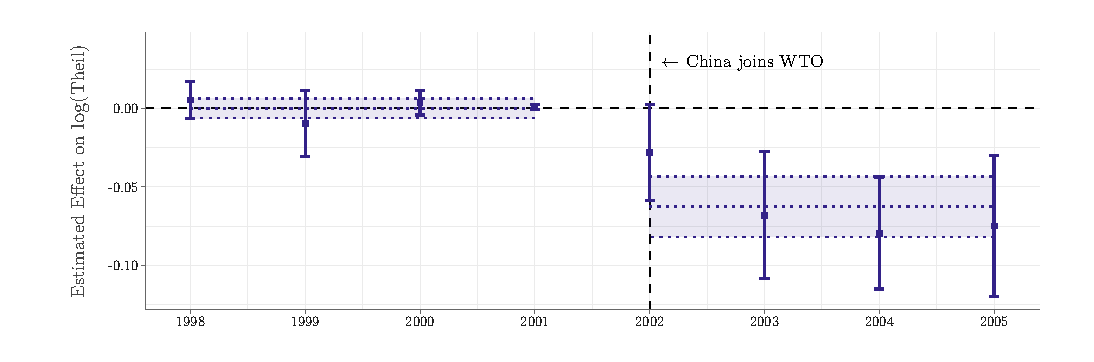
\includegraphics{../figures/trade-cce_est_interpolated.pdf}
    \end{adjustbox}
  \end{figure}
\end{frame}

\begin{frame}
  \begin{figure}
    \caption{Mediated Effect via A Decline in TFP Dispersion}
    \begin{adjustbox}{width=\textwidth}
      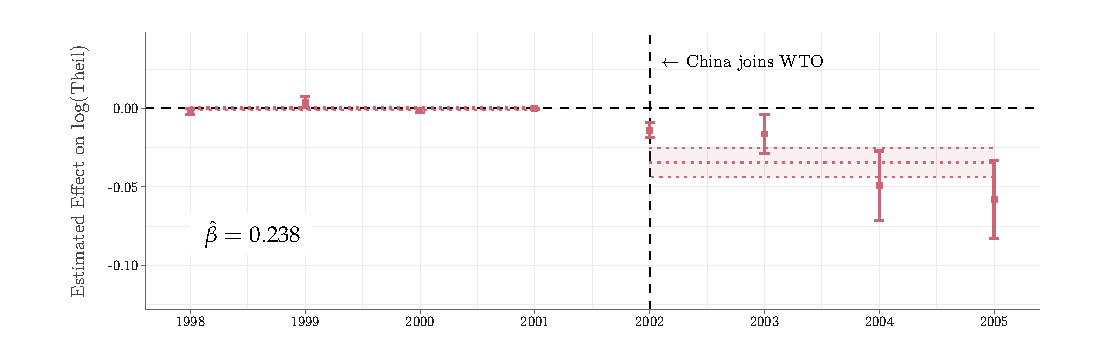
\includegraphics{../figures/trade-cce_mediated_est_interpolated.pdf}
    \end{adjustbox}
  \end{figure}
\end{frame}



\end{document}
